 
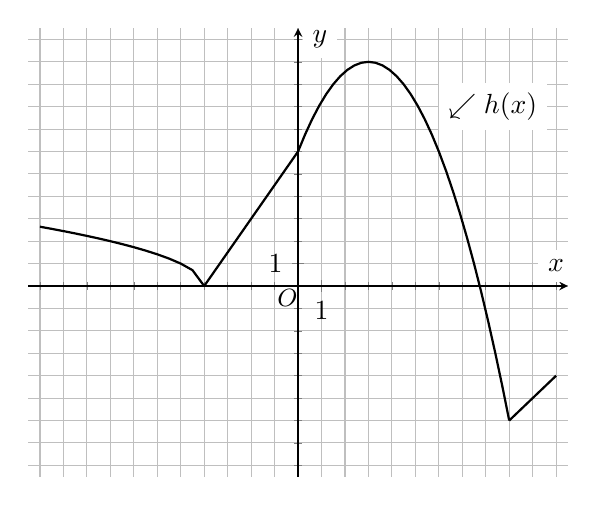
\begin{tikzpicture}
\begin{axis}[axis lines=center, xmin=-11.5, xmax=11.5, ymin=-8.5, ymax=11.5, grid=minor, grid style={thin, gray!50!white}, minor xtick={-11, -10, ..., 11}, minor ytick={-8, -7, ..., 11}, xtick={1}, ytick={1}, ]
\draw(axis cs:0.4,0.3)node[anchor=north east]{\small $O$}
(axis cs: 11,0.2)node[anchor=south, rectangle, fill=white, draw=white]{$x$} 
(axis cs: 0.2,11)node[anchor=west, rectangle, fill=white, draw=white]{$y$};
\addplot[thick,domain=-11:-4,samples=15,]{(-4-x)^.5};
\addplot[thick,domain=-4:0, samples=5,]{1.5*x+6};
\addplot[thick,domain=0:9, samples=31,]{-4*(x-3)^2/9+10};
\addplot[thick,domain=9:11, samples=5,]{x-15};
\draw(axis cs:6,8)node[anchor=west, rectangle, fill=white, draw=white]{$\swarrow h(x)$};
\end{axis}
\end{tikzpicture}\\
 The complete graph of the function $h$ is shown in the $xy$-plane above.  For what value of $x$ is the value of $h(x)$ at its maximum?


\ifsat
	\begin{enumerate}[label=\Alph*)]
		\item $3 $ % 
		\item $9 $ 
		\item $10 $ 
		\item $11 $
	\end{enumerate}
\else
\fi

\ifacteven
	\begin{enumerate}[label=\textbf{\Alph*.},itemsep=\fill,align=left]
		\setcounter{enumii}{5}
		\item $3 $ % 
		\item $9 $ 
		\item $10 $ 
		\addtocounter{enumii}{1}
		\item $11 $
		\item None of these. 
	\end{enumerate}
\else
\fi

\ifactodd
	\begin{enumerate}[label=\textbf{\Alph*.},itemsep=\fill,align=left]
		\item $3 $ % 
		\item $9 $ 
		\item $10 $ 
		\item $11 $
		\item None of these. 
	\end{enumerate}
\else
\fi

\ifgridin
 $3 $ % 
		
\else
\fi

